
\newpage

\section{Crystal structure of sodium chloride (NaCl)}
\label{sec:NaCl}

\subsection*{Structural Analysis}


In the following section, we are going to examine the crytsal structure of NaCl. Using the setup described in~\ref{chap:methods} we recieved the measured intensities as function of the angle $2\theta$. The corresponding graph, depicted in fig.~\ref{fig:Peaks}, shows multiple peaks, which result from diffractions at different Miller planes.  

\begin{figure}[ht]
    \centering
    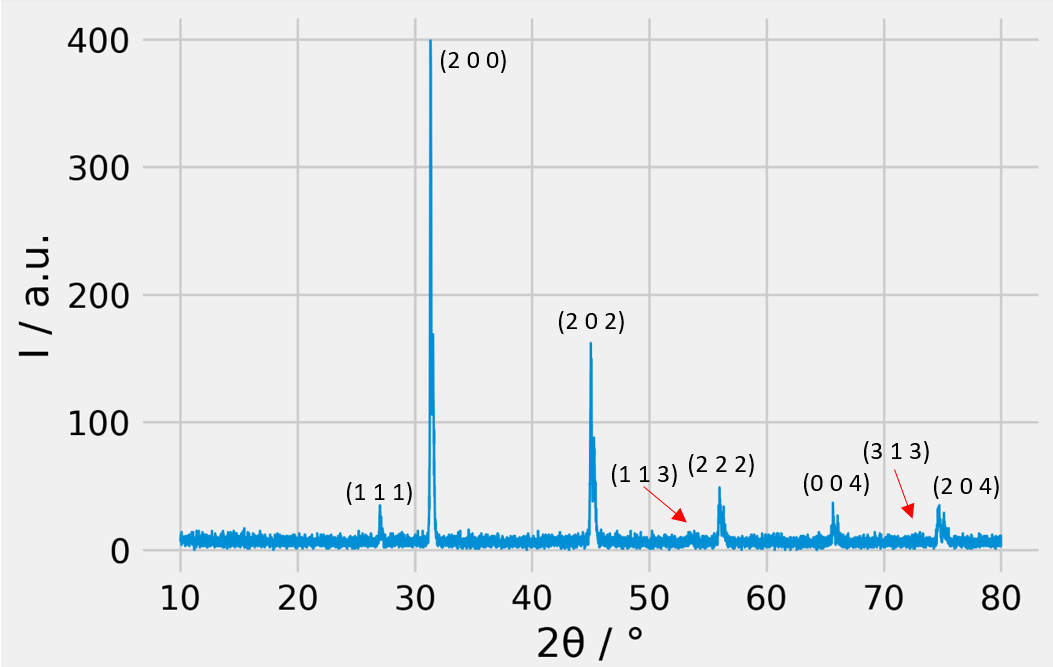
\includegraphics[angle = 90, width = 0.8\linewidth]{Bilder/Auswertung/NaCl/Ivs2thwIndices.png}
    \label{fig:Peaks}
    \caption{The intensity distribution is shown as a function of the angle $2\theta$. The visible and calculated Peaks are labeled with their corresponding Laue indices.}
\end{figure}

It should be noted, that each peak consists of two subpeaks due to the two slightly different wavelengths of the Cu-K$\alpha$1 line and the Cu-K$\alpha$2 line. Therefore, each peak was fitted, but only the values for the Cu-K$\alpha$1 line were taken in account for further calculations. The corresponding values for the full width at half maximum (FWHM) and the intensity of each peak are stated in tab.~\ref{tab:fitVals}.

\begin{table}[ht]
    \centering
    \begin{tabular}{c|c c c}
        \toprule
        Peak No. &  2$\theta_{fit}$ / \SIUnitSymbolDegree &  $I_{fit}$ / a.u. &   $FWHM$ / \SIUnitSymbolDegree \\
        \midrule
            1 &    27.24 &   0.05 &  0.11 \\
            2 &    31.56 &   0.86 &  0.12 \\
            3 &    45.24 &   0.48 &  0.16 \\
            4 &    53.62 &   0.03 &  0.18 \\
            5 &    56.21 &   0.15 &  0.19 \\
            6 &    65.91 &   0.10 &  0.22 \\
            7 &    72.70 &   0.02 &  0.24 \\
            8 &    74.91 &   0.17 &  0.25 \\
        \bottomrule
    \end{tabular}
    \caption{Fit values for each peak in the intensity distribution.}
    \label{tab:fitVals}
\end{table}

Subsequently, the peaks were indexed using the following relations: In order to see a reflex, Bragg's condition 
\begin{equation}
    2 d \sin\theta = m \lambda
    \label{eq411}
\end{equation}
has to be fulfilled. In cubic systems, the distance between to planes $d$ can be calculated simply as 
\begin{equation}
    d_{hkl} = \frac{a^2}{h^2+k^2+l^2}
    \label{eq412}
\end{equation}
with the Laue indices $h$, $k$ and $l$ and the lattice parameter $a$. Using $m=1$ equantions~\ref{eq411} and~\ref{eq:412} can be written together as 
\begin{equation}
    \sin^2\theta = (h^2+k^2+l^2) \frac{\lambda^2}{4a^2}.
\end{equation}
 Here, $c^{-1} := \frac{\lambda^2}{4a^2}$ is a constant parameter depending on the setup. Being reminded, that $(h^2+k^2+l^2) \in \mathbb{N}$ and knowing, that the smallest $2\theta$ is corresponding to small Laue indices, one can assign $h$,$k$,$l$ to $2\theta$, obtaining $a$ from
 \begin{equation}
    a = \sqrt{c}\frac{\lambda}{2}
 \end{equation}
 and $d$ from eq.~\ref{eq412}. All those values can be found in tab.~\ref{tab:latticeParams}.

 \begin{table}
    \centering
    \begin{tabular}{c | c c c c c c c}
        \toprule
        Peak No. &  2$\theta_{fit}$ / \SIUnitSymbolDegree &    $d$ / \SIUnitSymbolAngstrom &  $\sin^2(\theta)$ &  $\frac{\lambda^2}{4a^2}$ &  $h^2+k^2+l^2$ &    $a$ / \SIUnitSymbolAngstrom &   (h k l) \\
        \midrule
        1 &   27.240 & 3.271 & 0.055 &     0.018 &       3 & 5.666 & (1 1 1) \\
        2 &   31.563 & 2.832 & 0.074 &     0.018 &       4 & 5.665 & (0 0 2) \\
        3 &   45.241 & 2.003 & 0.148 &     0.018 &       8 & 5.665 & (2 0 2) \\
        4 &   53.618 & 1.708 & 0.203 &     0.018 &      11 & 5.665 & (1 1 3) \\
        5 &   56.208 & 1.635 & 0.222 &     0.018 &      12 & 5.665 & (2 2 2) \\
        6 &   65.905 & 1.416 & 0.296 &     0.018 &      16 & 5.665 & (0 0 4) \\
        7 &   72.705 & 1.300 & 0.351 &     0.018 &      19 & 5.665 & (3 1 3) \\
        8 &   74.912 & 1.267 & 0.370 &     0.018 &      20 & 5.665 & (2 0 4) \\
        \bottomrule
    \end{tabular}
    \caption{Lattice parameters and indices for each peak fitted.}
    \label{tab:latticeParams}
 \end{table}

Here, all found values for the lattice parameter \par  
\centerline{\boxed{$a = $ \SI{5.665}{\angstrom}},} \par 
differ only very slightly. Also, there is only a minor discrepancy to the value found in the literature of $a =$ \SI{5.64}{\angstrom}~\cite{Toreki2020}.  \par 
With the value $a$ found and keeping in mind, that we assume a cubic lattice, one can calculate the formula units for each unit cell $Z$ using the known density of NaCl $\rho = $\SI{2.17}{\gram \per \centi\metre^3} 
\begin{align}
    \rho &= \frac{m}{V} = \frac{Z M_M}{V_{uc}N_A} = \frac{Z M_M}{a^3 N_A} \\
    \Leftrightarrow Z &= \frac{\rho a^3 N_A}{M_M},
\end{align}
where $N_A$ is Avogadro's constant, $V_{uc}$ is the volume of a unit cell and $M_M =$\SI{58.44}{\gram \per \mol} is the molar mass of NaCl. These calculations lead to a value of \par 
\centerline{\boxed{$Z =$ \num{4}},} \par 
which is exactly what we expected for NaCl~\cite{Toreki2020}. When analyzing the reflection conditions of the indexed peaks from tab.~\ref{tab:latticeParams} we discovered, that NaCl has either to be of the point or space group $F23$, $Fm\overline{3}$, $F432$, $F\overline{4}3m$ or $Fm\overline{3}m$. The exact conditions fulfilled are marked in fig.~\ref{fig:reflexCond}.

\begin{figure}[ht]
    \centering
    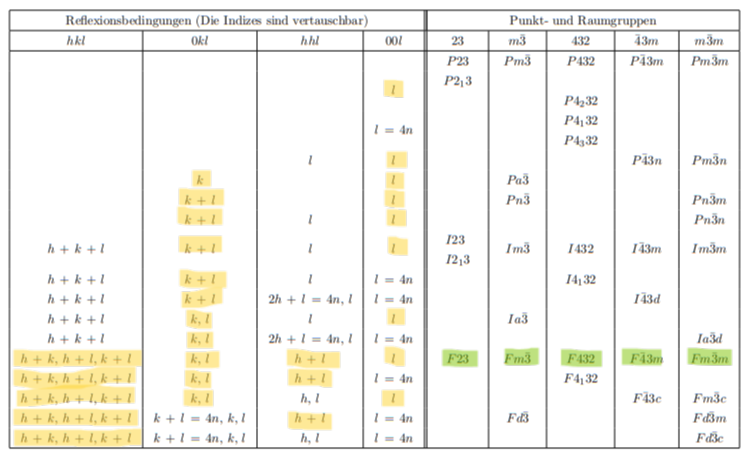
\includegraphics[angle = 90, width = 0.8 \linewidth]{Bilder/Auswertung/NaCl/table extinktion marked.png}
    \label{fig:reflexCond}
    \caption{For each of the reflex groups the fulfilled reflex conditions of the indexed peaks from tab.~\ref{tab:latticeParams} are marked in yellow. Subsequently, only a few point and space groups are left for the description of NaCl; they are marked in green. Table from~\cite{Aroyo2016}}
\end{figure}

Because further calculations would be far to complicated, we were hinted by the handout for the experiment, that the actual space group is $Fm\overline{3}m$. Remembering, that we found $Z=4$ and our structure is cubic, we assume, that NaCl is a face centered cubic (fcc) with a two atom basis (Na and Cl). Anyhow, we still do not know the basis. Therefore, two structure models $\mathbf{A}$ and $\mathbf{B}$ were suggested, where the coordinates of the atoms are $Na_{\mathbf{A}} = (0,0,0)$, $Cl_{\mathbf{A}} = (0.5,0.5,0.5)$ and $Na_{\mathbf{B}} = (0,0,0)$, $Cl_{\mathbf{B}} = (0.25,0.25,0.25)$, respectively. Due to the fcc-structure additional Na atoms are on positions $(0,0.5,0.5)$, $(0.5,0.5,0)$ and $(0.5,0,0.5)$ and Cl atoms on positions $(0,0,0.5)$, $(0,0.5,0)$ and $(0.5,0,0)$ for model \textbf{A} and $(0.75,0.5,0.5)$, $(0.5,0.5,0.75)$ and $(0.5,0.75,0.5)$ for model \textbf{B}, respectively. The intensity for the reflection on the plane (hkl) is proportional to 
\begin{equation}
    I_{hkl} \propto KALPEHT|F_{hkl}|^2,
\end{equation}
where $K$ is a scaling factor, $A$ is the absorption factor, $L$ is the Lorentz factor, $P$ is the polarisation factor, $E$ is the extinction factor, $H$ is the area frequency factor, $T$ is the Debye-Waller temperature factor and $|F_{hkl}|^2$ is the structure factor. Here, $K$ will be canceled out by normalizing the intensities to the (2 0 0) plane intensity and $A$, $E$ and $T$ are considered to be equal to 1. $H$ can simply be counted and the further factors can be calculated as 
\begin{align}
    L(\theta) &= \frac{1}{\sin(\theta)\cos(\theta)} \\
    P(\theta) &= \frac{1+\cos^2(2\theta)}{2} \\
    F_{hkl} &= \sum_{j=1}^{N} f_j \exp[2\pi i\cdot (hx_j+ky_j+lz_j)]\mathrm{, with} \\
    f\left(\frac{\sin(\theta)}{\lambda}\right) &= \sum_{j=1}^{4} \left[a_i\exp\left\{-b_i\left(\frac{\sin(\theta)}{\lambda}\right)^2\right\}\right] + c, \\
\end{align}
where the $a_j$, $b_j$ and $c$ are constants for a given element. The intensities for the measurement $I_{meas,norm}$, model \textbf{A} $I_{\mathbf{A},norm}$ and model \textbf{B} $I_{\mathbf{B},norm}$, all normalized to the (0 0 2) reflection, are shown in tab.~\ref{tab:ints}. The calculated factors for the intensities of the models are shown in tab.~\ref{tab:intParams}. 

\begin{table}
    \centering
    \begin{tabular}{c|c c c c}
        \toprule
         Peak No. &   (h k l) &  $I_{meas,norm}$ / a.u. &  $I_{\mathbf{A},norm}$ / a.u. &   $I_{\mathbf{B},norm}$ / a.u. \\
        \midrule
               1 & (1 1 1) &        0.060 &     0.074 &     5.583 \\
               2 & (0 0 2) &        1.000 &     1.000 &     1.000 \\
               3 & (2 0 2) &        0.557 &     0.923 &     0.990 \\
               4 & (1 1 3) &        0.035 &     0.031 &     1.322 \\
               5 & (2 2 2) &        0.178 &     0.364 &     0.058 \\
               6 & (0 0 4) &        0.118 &     0.185 &     1.126 \\
               7 & (3 1 3) &        0.027 &     0.021 &     0.589 \\
               8 & (2 0 4) &        0.195 &     0.551 &     0.545 \\
        \bottomrule
        \end{tabular}
        \caption{The intensities of the measurement and for the calculated models \textbf{A} and \textbf{B}, all normalized to the (0 0 2) reflection.}
        \label{tab:ints}
\end{table}

\begin{table}
    \centering
    \begin{tabular}{c|c c c c c c c c c}
        \toprule
         Peak No. &  2$\theta_{fit}$ / \SIUnitSymbolDegree &  (h k l) &  $L(\theta)$ &  $P(\theta)$ &  $H$ &   $f_{Na}$ &    $f_{Cl}$ &   $|F_{hkl,\mathbf{A}}|^2$ &   $|F_{hkl,\mathbf{B}}|^2$ \\
        \midrule
               1 &   27.240 & (1 1 1) & 4.369 & 0.895 &  8 & 8.992 & 13.633 &  344.618 & 4267.321 \\
               2 &   31.563 & (0 0 2) & 3.821 & 0.863 &  6 & 8.693 & 12.769 & 7369.392 & 1209.013 \\
               3 &   45.241 & (2 0 2) & 2.817 & 0.748 & 12 & 7.651 & 10.593 & 5325.700 &  936.608 \\
               4 &   53.618 & (1 1 3) & 2.484 & 0.676 & 24 & 7.003 &  9.660 &  112.967 &  784.627 \\
               5 &   56.208 & (2 2 2) & 2.407 & 0.655 &  8 & 6.808 &  9.422 & 4214.437 &  109.347 \\
               6 &   65.905 & (0 0 4) & 2.191 & 0.583 &  6 & 6.115 &  8.700 & 3512.050 & 3512.050 \\
               7 &   72.705 & (3 1 3) & 2.095 & 0.544 & 24 & 5.675 &  8.318 &  111.841 &  515.219 \\
               8 &   74.912 & (2 0 4) & 2.071 & 0.534 & 24 & 5.540 &  8.211 & 3025.663 &  491.116 \\
        \bottomrule
        \end{tabular}
        \caption{Calculated parameters needed for calculating the intensities of models \textbf{A} and \textbf{B}.}
        \label{tab:intParams}
\end{table}

In fig.~\ref{fig:histoInts}, the intensities of each peak for each model are displayed as a histogram. In some cases, the difference of the models to the measurement are almost the same. However, for some peaks (e.g. No.4,6,7) model \textbf{A} suits the measurement far better than model \textbf{B}. This fulfills our expectations since model \textbf{A} is the model the literature states for NaCl~\cite{Toreki2020}.

\begin{figure}[ht]
    \centering
    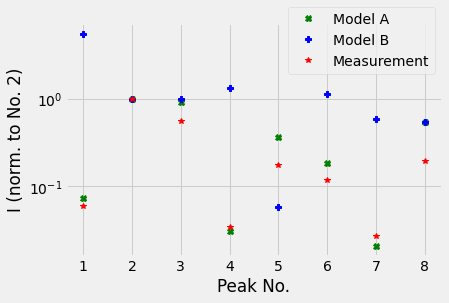
\includegraphics[width = 0.8\linewidth]{Bilder/Auswertung/NaCl/IntsModels.png}
    \label{fig:histoInts}
    \caption{The intensities for the measurement (red) an for both calculated models \textbf{A} (green) and \textbf{B} (blue) are displayed as a histogram. It is clear, that model \textbf{A} suits the measurement far better than model \textbf{B}.}
\end{figure}

\subsection*{Device Function}

Because of the high cristallinity of NaCl, the influence of the probe regarding the broadening of the peaks can be neglecteg. Therefore, it is possible to directly determine the device function using the formula for the FWHM 
\begin{equation}
    FWHM(\theta) = \sqrt{U \tan^2(\theta) + V \tan(\theta) + W}.
\end{equation}
A fit was calculated using the values for $FWHM(\theta)$ from tab.~\ref{tab:fitVals}. The values found are \par 
\centerline{\boxed{$U =$ \num{2.91e-5}, \quad $V =$ \num{6.04e-9}, \quad $W =$ \num{2.31e-6}.}} \par
The fitted device function aligns the data perfectly, as can be seen in fig.~\ref{fig:devFct}. Therefore, the assumption of a neglectable probe influence seems to be correct.

\begin{figure}[ht]
    \centering
    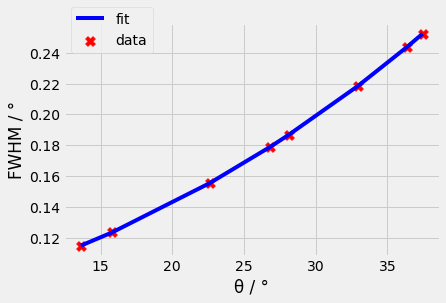
\includegraphics[width = 0.8\linewidth]{Bilder/Auswertung/NaCl/deviceFct.png}
    \label{fig:devFct}
    \caption{The fitted device function describes the correlation between the FWHM and the angle $\theta$. Although simplifications have been made, the fit aligns perfectly with the data.}
\end{figure}
